% conclusion.tex
% Section 5: Synthesis and Outlook

\section{Synthesis and Outlook}
\label{sec:synthesis}

\subsection{Combining Output and System Validity}
\label{sec:synthesis:compose}

Output validity is a claim about the learned object itself. System validity
connects a result obtained in a designed game to the objective outside that
game:
\[
\begin{aligned}
\text{output validity:}\qquad
&\widehat{x} \quad\Longrightarrow?\quad P_\Gamma(\widehat{x}),\\
\text{system validity:}\qquad
&P_{\Gamma_Q}(x) \quad\Longrightarrow?\quad Q(x),
\end{aligned}
\]
where $\Longrightarrow?$ marks an implication whose validity is the object of
study, $P_\Gamma$ is a property defined for a game $\Gamma$, and $Q$ is the
objective around which $\Gamma_Q$ was designed.

Composition requires the same object, game, and domain in both claims. Setting
$x=\widehat{x}$ and $\Gamma=\Gamma_Q$ gives
\[
\widehat{x} \;\Longrightarrow\; P_{\Gamma_Q}(\widehat{x}) \;\Longrightarrow\;
Q(\widehat{x}).
\]
Algorithmic pricing illustrates why the conditions matter. Each pricing
algorithm may satisfy a local criterion while the market fails an external
welfare objective. The local property concerns one firm maximizing its own
profit. The system objective concerns the joint market outcome and includes
consumers who are affected parties outside that local optimization.

For an output property defined through deviations, finite search generally
provides a lower bound on the largest gain. Assume that the target class contains
a null deviation, and define
$g_\Gamma(x)=\sup_{d\in\mathcal{D}_\Gamma(x)}\Delta_\Gamma(x,d)$ as the largest
gain over that class. A search that returns some $\widehat d$ establishes the
lower bound $g_\Gamma(x)\ge\Delta_\Gamma(x,\widehat d)$.
An upper bound on $g_\Gamma$ requires a guarantee on the search itself: if
$\Delta_\Gamma(x,\widehat d)\ge g_\Gamma(x)-\epsilon$, then observing
$\Delta_\Gamma(x,\widehat d)\le\eta$ yields $g_\Gamma(x)\le\eta+\epsilon$.
Without such a guarantee, the observation controls only the searched class.
Figure~\ref{fig:candidate-counterexample} summarizes this asymmetry between
finite counterexample search and a claim over the full deviation class.

Identification claims instead use observations and maintained assumptions to
define an identified set. They need not involve a searched deviation class.

\begin{figure}[pos=h]
\centering
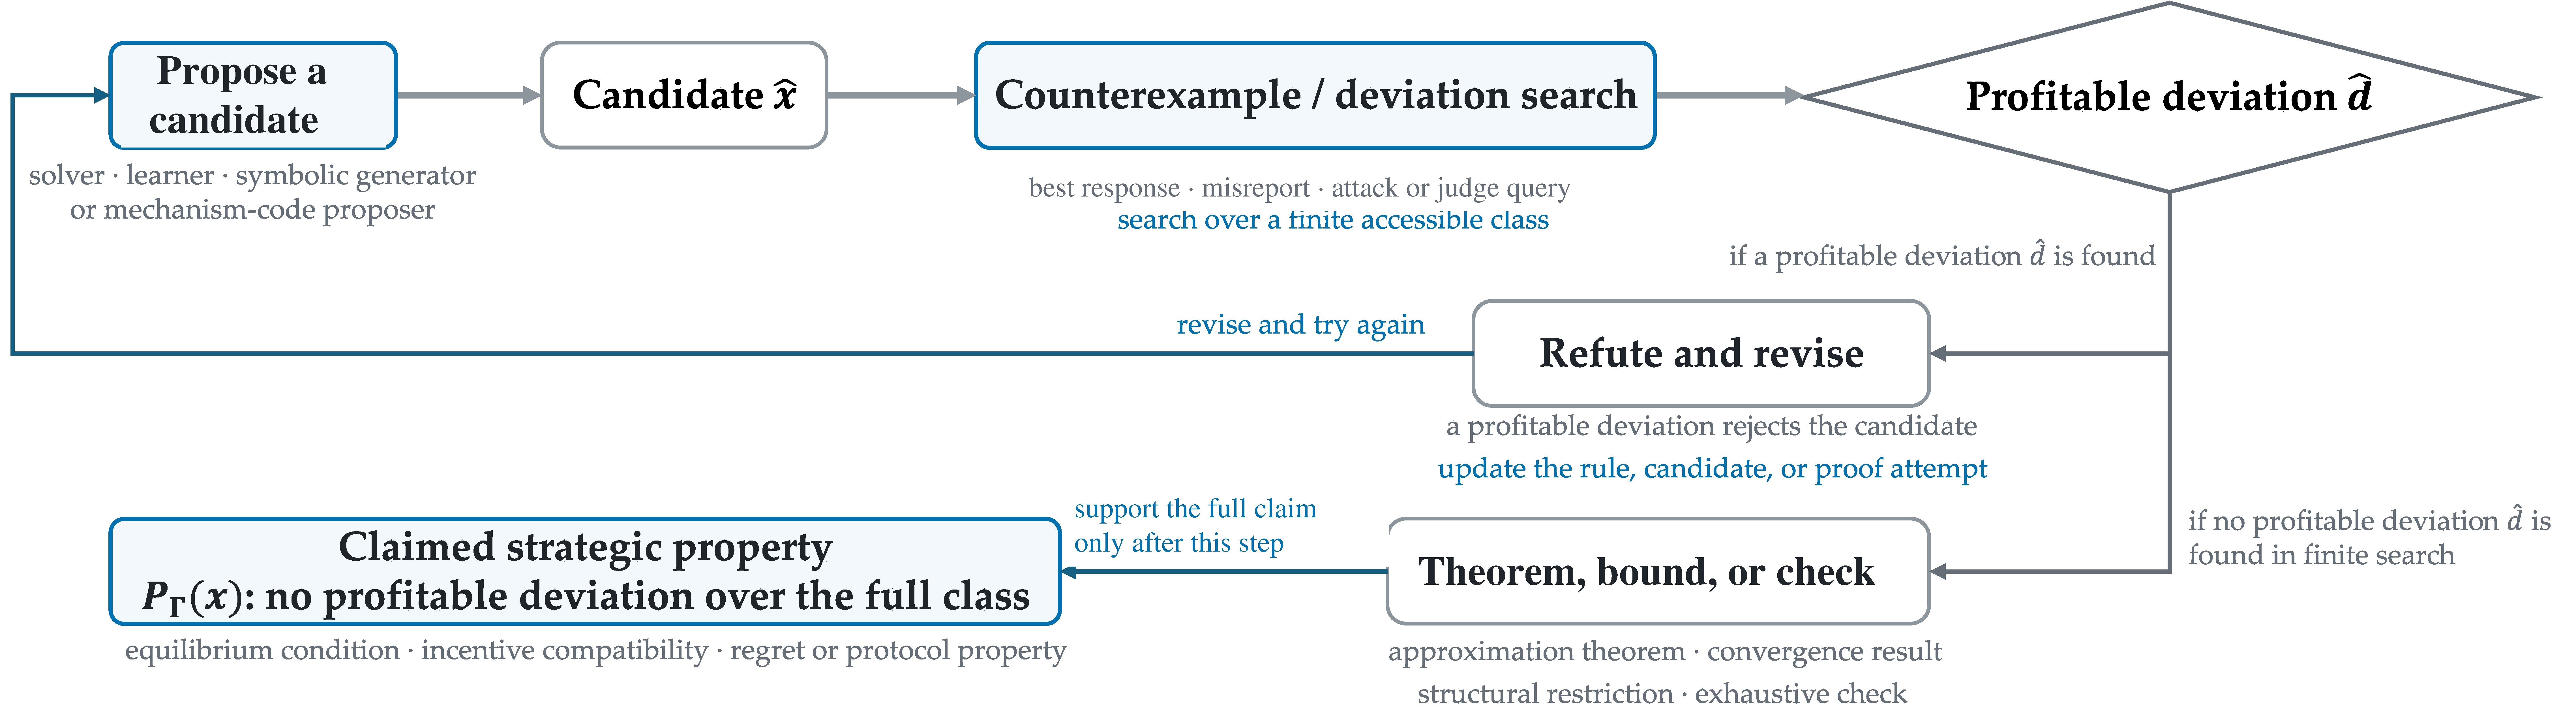
\includegraphics[width=\textwidth]{figure/fig4-candidate-counterexample.pdf}
\caption{Finite evaluation of a deviation-defined property. A method proposes a
candidate and searches for a profitable deviation in an accessible class. A
discovered deviation refutes the candidate. If the search finds none, a claim
over the target class requires a theorem, bound, or structural argument that
controls the alternatives not searched. Identification and system-validity
claims require different arguments.}
\label{fig:candidate-counterexample}
\end{figure}

\subsection{What Each Domain Contributes}
\label{sec:synthesis:map}

Table~\ref{tab:domain-map} summarizes the primary limitation in each domain and
the additional argument needed for the target claim.

Broader search and response oracles address coverage, whereas identification
depends on new information or maintained restrictions. Cross-game variation,
exploration, and logging can reveal otherwise unobserved counterfactuals.
Pessimistic completion converts counterfactuals that remain unidentified into
conservative bounds.

\begin{table}[htbp]
\centering
\caption{The six domains, the question each makes concrete, and what connects
finite evidence to the target claim.}
\label{tab:domain-map}
\begin{tabularx}{\textwidth}{@{}p{2.6cm} p{2.1cm} p{2.0cm} Y@{}}
\toprule
\textbf{Domain} & \textbf{Question} & \textbf{Primary limit} & \textbf{Additional argument} \\
\midrule
Constructive equilibrium (\S\ref{sec:ai4gt:equilibrium})
& Output validity & Coverage
& Duality in the zero-sum case; the regret decomposition; safe-resolving bounds; an executable derivation \\
\addlinespace
Strategic inference (\S\ref{sec:ai4gt:inference})
& Output validity & Identification
& Falsifiability plus recoverability; cross-game and cross-environment variation; maintained restrictions \\
\addlinespace
Mechanism design (\S\ref{sec:ai4gt:mechanism})
& Output validity under response & Coverage
& Membership in a truthful family; post-processing with a regularity bound
carrying a finite grid to a continuous domain; a stated deployment-domain
argument where participation or reports shift \\
\addlinespace
Strategic evaluation (\S\ref{sec:gt4ai:evaluation})
& Output validity under response & Coverage
& Response-oracle expansion over a stated policy class, or a certified robustness radius \\
\addlinespace
Designed games as evidence (\S\ref{sec:gt4ai:training})
& System validity & Designed-game scope
& Protocol theorems with stated bounds on adversary and judge; an argument that the constructed objective is the intended one \\
\addlinespace
Deployment governance (\S\ref{sec:gt4ai:governance})
& System validity & Coverage \emph{and} identification
& Correlated-equilibrium restrictions from low calibrated regret; pessimistic completion; an external welfare or legal benchmark \\
\bottomrule
\end{tabularx}
\end{table}

\begin{table}[htbp]
\centering
\caption{Four forms of evidence used in the surveyed domains, together with the
claims and assumptions associated with each. A system may combine several
forms.}
\label{tab:strategic-evidence}
\footnotesize
\setlength{\tabcolsep}{3.5pt}
\renewcommand{\arraystretch}{1.25}

\begin{tabularx}{\textwidth}{
    >{\raggedright\arraybackslash}p{0.15\textwidth}
    >{\raggedright\arraybackslash}p{0.22\textwidth}
    Y
    Y
}
\toprule
\textbf{Evidence basis}
& \textbf{Claim supported}
& \textbf{Scope and assumptions}
& \textbf{Conclusion and cost}
\\
\midrule

Machine-checked derivation
& Equilibrium or approximation property of a strategy profile or synthesized
algorithm
& Explicit formal game or algorithm; sound encoding and trusted checker
& Deductive result for the encoded statement; construction and checking cost
\cite{PrimeNash2025,LegoNE2025}
\\

\addlinespace

Structural theorem
& Incentive compatibility or strategy-proofness of a mechanism
& Membership in the theorem's representation family; domain and regularity
assumptions
& Exact or bounded theorem-specific result; representation and post-processing
cost \cite{Shen2019,Duan2023,Duetting2024}
\\

\addlinespace

Protocol theorem
& Soundness, completeness, or a winning-strategy result for an interactive
protocol
& Specified roles and information; bounds on the judge, adversary, and available
computation
& Result within the protocol model; verifier resources
\cite{Irving2018,BrownCohen2023}
\\

\addlinespace

Behavioral statistical test
& Regret or another specified property of a deployed policy
& Logged play and assumptions on sampling, exploration, and the market
& Probabilistic result for the data-generating process; sample and computation
cost \cite{HartlineLongZhang2024,HartlineWangZhang2025}
\\
\bottomrule
\end{tabularx}
\end{table}
\FloatBarrier

\subsection{Research Priorities}
\label{sec:synthesis:open}

For each empirical estimate of strategic performance, reproducible comparisons
require authors to identify the alternative class and explain how it relates to
the target claim. Cost comparisons should report training and evaluation as
well as per-instance inference.

Strategic inference should make greater use of partial identification. When
several latent explanations fit observed play, the relevant question is which
counterfactual conclusions hold across the identified set. Pessimistic
completion in deployment auditing provides one example of this approach.

Claims about training and oversight protocols should state the modeled resource
and information bounds on every participant. These assumptions determine what
the designed game establishes and should appear in the main statement of the
result.

Deployment studies also need evaluation domains that account for participant
responses. This requires a model or audit of how those responses select the
post-deployment cases to which the property is claimed to extend.
